\documentclass[border=3pt]{standalone}
% Preâmbulo compartilhado pelos diagramas TikZ da aula 11 (Localização por Grade e Monte Carlo)
\usepackage[T1]{fontenc}
\usepackage[utf8]{inputenc}
\usepackage{lmodern}
\usepackage{amsmath}
\usepackage{xcolor}
\usepackage{tikz}
\usetikzlibrary{arrows.meta,angles,quotes,decorations.pathmorphing,calc,
                positioning,shapes.geometric,shapes.misc,backgrounds,fit,
                math}

% Paleta (mesma dos SVGs originais)
\definecolor{dblue}{HTML}{2A5B8C}
\definecolor{dorange}{HTML}{B3541E}
\definecolor{dgreen}{HTML}{4A7C59}
\definecolor{dred}{HTML}{9C4B4B}
\definecolor{dcream}{HTML}{F4F1EA}
\definecolor{dshade}{HTML}{DDD7C9}

% Função gaussiana (não normalizada por padrão de escala visual)
\pgfmathdeclarefunction{gauss}{3}{%
  \pgfmathparse{1/(#3*sqrt(2*pi))*exp(-((#1-#2)^2)/(2*#3^2))}%
}

% Estilos comuns (prefixo d... para não colidir com chaves internas do pgf)
\tikzset{
  >={Stealth[length=2mm]},
  dguide/.style={gray!55, dashed, line width=0.4pt},
  daxis/.style={gray!60, line width=0.7pt, ->},
  dbody/.style={fill=black!3, draw=black!80, line width=1pt},
  dacc/.style={draw=dblue, line width=1pt},
  dlbl/.style={black!55, font=\small},
  dsub/.style={black!45, font=\footnotesize},
  dstate/.style={circle, draw=black!80, fill=dcream, line width=1pt,
                 minimum size=17mm, font=\large, inner sep=1pt},
  dobs/.style={circle, draw=black!80, fill=dshade, line width=1pt,
               minimum size=14mm, font=\large, inner sep=1pt},
  dbox/.style={rounded corners=2pt, draw=black!80, fill=dcream, line width=1pt,
               align=center, inner sep=6pt},
  dop/.style={circle, draw=black!80, fill=white, line width=1pt,
              minimum size=6mm, inner sep=0pt, font=\small},
  dtrans/.style={->, dblue, line width=1pt},
  dmeas/.style={->, dorange, line width=1pt},
  dcurve/.style={line width=1pt, dblue},
  dcurveb/.style={line width=1.4pt, dorange},
}

\begin{document}
\hyphenpenalty=10000 \exhyphenpenalty=10000 \tolerance=9999 \emergencystretch=3em
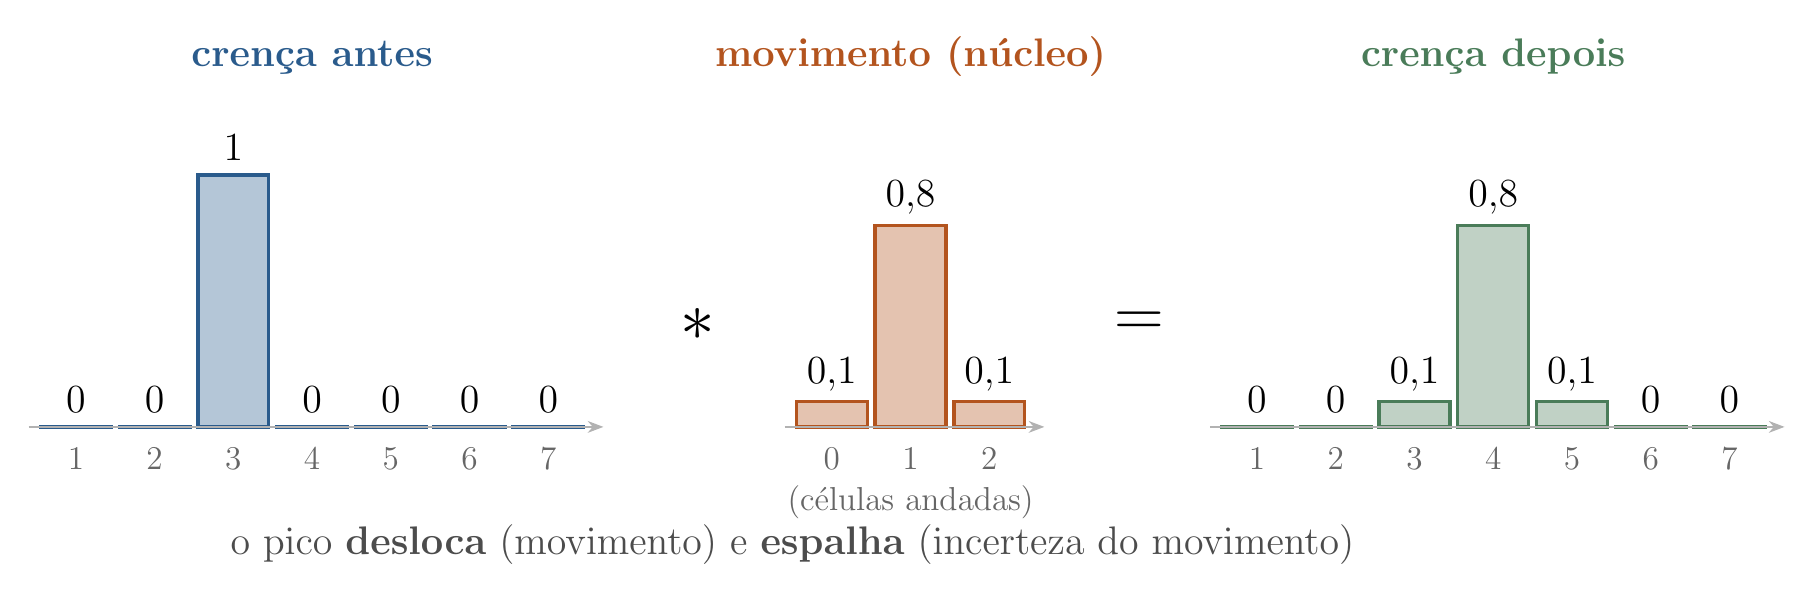
\begin{tikzpicture}[x=1cm,y=1cm]
  \def\esc{3.2}
  \expandafter\def\csname lbl0\endcsname{0}\expandafter\def\csname lbl0.1\endcsname{0,1}\expandafter\def\csname lbl0.8\endcsname{0,8}\expandafter\def\csname lbl1\endcsname{1}
  % bars(ox, valores, cor, deslocamento-do-índice inicial)
  \newcommand{\barras}[4]{% ox, cor, lista de alturas, primeiro índice
    \foreach \h [count=\i from 0] in {#3} {
      \fill[#2!35!white, draw=#2, line width=1.2pt] ({#1+\i*1.0+0.05},0) rectangle ({#1+\i*1.0+0.95},{\esc*\h+0.001});
      \node[font=\Large] at ({#1+\i*1.0+0.5},{\esc*\h+0.35}) {\csname lbl\h\endcsname};
      \node[font=\large, black!60] at ({#1+\i*1.0+0.5},-0.4) {\pgfmathtruncatemacro{\ix}{#4+\i}\ix};
    }
    \draw[daxis] ({#1-0.1},0) -- ({#1+7.2},0);
  }
  % crença antes
  \node[font=\Large\bfseries, dblue] at (3.5,4.7) {crença antes};
  \barras{0}{dblue}{0,0,1,0,0,0,0}{1}
  \node[font=\Huge\bfseries] at (8.4,1.3) {$\ast$};
  % núcleo
  \node[font=\Large\bfseries, dorange] at (11.1,4.7) {movimento (núcleo)};
  \foreach \h/\d [count=\i from 0] in {0.1/0,0.8/1,0.1/2} {
    \fill[dorange!35!white, draw=dorange, line width=1.2pt] ({9.6+\i*1.0+0.05},0) rectangle ({9.6+\i*1.0+0.95},{\esc*\h+0.001});
    \node[font=\Large] at ({9.6+\i*1.0+0.5},{\esc*\h+0.35}) {\ifnum\i=1 0,8\else 0,1\fi};
    \node[font=\large, black!60] at ({9.6+\i*1.0+0.5},-0.4) {\d};
  }
  \draw[daxis] (9.5,0) -- (12.8,0);
  \node[font=\large, black!60] at (11.1,-0.95) {(células andadas)};
  \node[font=\Huge\bfseries] at (14.0,1.3) {$=$};
  % crença depois
  \node[font=\Large\bfseries, dgreen] at (18.5,4.7) {crença depois};
  \barras{15}{dgreen}{0,0,0.1,0.8,0.1,0,0}{1}
  \node[font=\Large, black!70] at (9.6,-1.5) {o pico \textbf{desloca} (movimento) e \textbf{espalha} (incerteza do movimento)};
\end{tikzpicture}
\end{document}
